
%(BEGIN_QUESTION)
% Copyright 2007, Tony R. Kuphaldt, released under the Creative Commons Attribution License (v 1.0)
% This means you may do almost anything with this work of mine, so long as you give me proper credit

Since liquid level can only change in a vessel if there is an imbalance of inlet and outlet flow rates, would this system be practical to achieve steady liquid level control?  Explain why or why not.

$$\includegraphics[width=15.5cm]{i01749x01.eps}$$

Note: the philosophy behind this control system is a principle known as {\it mass balance}, and it is a very valid principle.  Explain what the principle of ``mass balance'' is, and how it is implied in the design of this control system.

\vskip 10pt

Also, mark the SP and PV inputs of the controller in this system with ``+'' and ``$-$'' symbols as appropriate to show the correct controller action.

\vskip 20pt \vbox{\hrule \hbox{\strut \vrule{} {\bf Suggestions for Socratic discussion} \vrule} \hrule}

\begin{itemize}
\item{} Explain why the control system as shown is impractical for real-life use, despite the fact that it does represent a very effective and important control strategy frequently used in industry.
\item{} Explain what ``Fieldbus'' instruments are, and how they differ from traditional instrumentation.
\item{} How will this control system respond if the ``wild'' flow transmitter fails with a high signal?
\item{} How will this control system respond if the ``drain'' flow transmitter fails with a high signal?
\item{} How will this control system respond if the control valve's air supply fails?
\item{} How will this control system respond if the ``wild'' flow line becomes partially plugged?
\item{} How will this control system respond if the ``drain'' flow line becomes partially plugged?
\item{} Are there any loads unaccounted for in this feedforward control strategy?
\end{itemize}

\underbar{file i01749}
%(END_QUESTION)





%(BEGIN_ANSWER)

In theory, this {\it feedforward} system would work to hold the liquid level absolutely constant, because it will try to maintain flow out equal to flow in (mass out {\it balances} mass in).  However, there are some practical reasons why it would not work.

\vskip 10pt

The controller needs to be {\it reverse action}, assuming a signal-to-open control valve:

$$\includegraphics[width=15.5cm]{i01749x02.eps}$$

The ``+'' symbol at the SP input of the controller tells us there is a non-inverting relationship between the SP input and the controller output.  The ``$-$'' symbol at the PV input of the controller tells us there is an inverting relationship between the PV input and the controller output.  Both of these characteristics are consistent with what we call ``reverse'' action in a loop controller.

%(END_ANSWER)





%(BEGIN_NOTES)

Consider what would happen if the two flow transmitters were not calibrated precisely the same.  This would create an imbalance of inlet/outlet flow, resulting in the liquid level ``integrating'' either up or down until the vessel either overflowed or ran dry, respectively.  Also, consider what would happen if a leak occurred.  Since the leak would remain undetected by the system, the vessel would slowly run empty and the controller would take no corrective action.

However, the advantages of feedforward control cannot be dismissed, even though this particular system is impractical.  By measuring the load(s) in a process and taking corrective action immediately in response to changes in load, the main process variable (liquid level, in this case) ideally sees no upset, just as the master control loop in a cascade system ideally sees no upset following load changes in the slave loop.  The technical term for this strategy is {\it load balancing}: when input and output loads are maintained in a state of equality, so that the controlled variable remains steady.

\vfil \eject

\noindent
{\bf Prep Quiz:}

{\it Mass balance} is a phrase meaning \underbar{what} in the context of process control?

\begin{itemize}
\item{} When the total mass output by a process is precisely equal to setpoint
\vskip 5pt 
\item{} When all the overshoots of setpoint balance out all the undershoots of setpoint
\vskip 5pt 
\item{} When the total material flowrate in equals the total material flowrate out
\vskip 5pt 
\item{} When the output signal of a loop controller is equal to the input (PV) signal
\vskip 5pt 
\item{} The precise measurement of material mass using a balance-scale instrument
\vskip 5pt 
\item{} It is a synonym for {\it force-balance} when referencing pneumatic instruments
\end{itemize}

%INDEX% Control, strategies: feedforward

%(END_NOTES)


